% Critical Difference (CD) Diagram
% k = 9 models, N = 24 evaluation blocks (12 assets x 2 forecast horizons)
% Primary source: results/benchmark/global_summary/tables/global_ranking_aggregated.csv
% Post-hoc test: Holm--Wilcoxon (alpha = 0.05)
% Non-significant pairs (holm_wilcoxon.csv, significant=False):
%   iTransformer -- TimeXer   (p_holm = 0.4800)
%   DLinear      -- N-HiTS    (p_holm = 0.5287)
%   TimesNet     -- Autoformer (p_holm = 0.5287)
% Nemenyi CD = q_{0.05}(9) * sqrt(k(k+1)/(6N))
%            = 3.102 * sqrt(90/144) = 2.4507  [reference bracket only]
%
% x-coordinate mapping:  x(r) = (r - 1) * 1.5  cm
%   ModernTCN    rank 1.3333  ->  x = 0.5000
%   PatchTST     rank 2.0000  ->  x = 1.5000
%   iTransformer rank 3.6667  ->  x = 4.0000
%   TimeXer      rank 4.2917  ->  x = 4.9375
%   DLinear      rank 4.9583  ->  x = 5.9375
%   N-HiTS       rank 5.2500  ->  x = 6.3750
%   TimesNet     rank 7.7083  ->  x = 10.0625
%   Autoformer   rank 7.8333  ->  x = 10.2500
%   LSTM         rank 7.9583  ->  x = 10.4375
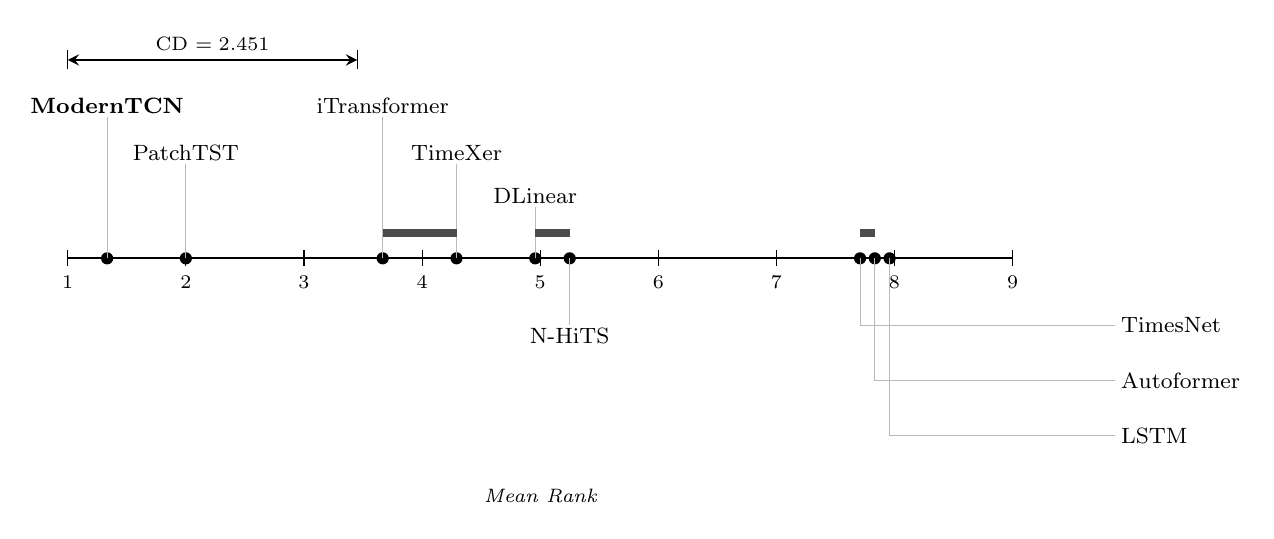
\begin{tikzpicture}[font=\small]

% =====================================================================
% Horizontal rank axis  (rank 1 = left/best, rank 9 = right/worst)
% =====================================================================
\draw[thick] (0,0) -- (12,0);

% Integer rank tick marks and labels
\foreach \r in {1,...,9}{
  \pgfmathsetmacro{\xt}{(\r-1)*1.5}
  \draw (\xt, 0.10) -- (\xt,-0.10);
  \node[below, font=\scriptsize] at (\xt,-0.10) {\r};
}

% =====================================================================
% Model dot markers at exact mean-rank positions
% =====================================================================
\foreach \xm in {0.5000, 1.5000, 4.0000, 4.9375, 5.9375,
                 6.3750, 10.0625, 10.2500, 10.4375}{
  \fill[black] (\xm,0) circle[radius=2.2pt];
}

% =====================================================================
% Top-half models: vertical stems + labels ABOVE axis
% Heights alternated to prevent label overlap
% =====================================================================

% ModernTCN   rank=1.3333   x=0.5000   h=1.8
\draw[gray!55,thin] (0.5000,0) -- (0.5000,1.8);
\node[above, inner sep=1pt, font=\footnotesize\bfseries]
  at (0.5000,1.8) {ModernTCN};

% PatchTST    rank=2.0000   x=1.5000   h=1.2
\draw[gray!55,thin] (1.5000,0) -- (1.5000,1.2);
\node[above, inner sep=1pt, font=\footnotesize]
  at (1.5000,1.2) {PatchTST};

% iTransformer   rank=3.6667   x=4.0000   h=1.8
\draw[gray!55,thin] (4.0000,0) -- (4.0000,1.8);
\node[above, inner sep=1pt, font=\footnotesize]
  at (4.0000,1.8) {iTransformer};

% TimeXer   rank=4.2917   x=4.9375   h=1.2
\draw[gray!55,thin] (4.9375,0) -- (4.9375,1.2);
\node[above, inner sep=1pt, font=\footnotesize]
  at (4.9375,1.2) {TimeXer};

% DLinear   rank=4.9583   x=5.9375   h=0.65
\draw[gray!55,thin] (5.9375,0) -- (5.9375,0.65);
\node[above, inner sep=1pt, font=\footnotesize]
  at (5.9375,0.65) {DLinear};

% =====================================================================
% Bottom-half models: stems + labels BELOW axis
% =====================================================================

% N-HiTS   rank=5.2500   x=6.3750   depth=0.85
\draw[gray!55,thin] (6.3750,0) -- (6.3750,-0.85);
\node[below, inner sep=1pt, font=\footnotesize]
  at (6.3750,-0.85) {N-HiTS};

% TimesNet / Autoformer / LSTM are within 0.375 cm of each other.
% Use staggered depths + horizontal leaders to a right-margin label column.

% TimesNet   rank=7.7083   x=10.0625   depth=0.85 -> leader to x=13.3
\draw[gray!55,thin] (10.0625,0) -- (10.0625,-0.85) -- (13.3,-0.85);
\node[right, inner sep=2pt, font=\footnotesize] at (13.3,-0.85) {TimesNet};

% Autoformer   rank=7.8333   x=10.2500   depth=1.55 -> leader to x=13.3
\draw[gray!55,thin] (10.2500,0) -- (10.2500,-1.55) -- (13.3,-1.55);
\node[right, inner sep=2pt, font=\footnotesize] at (13.3,-1.55) {Autoformer};

% LSTM   rank=7.9583   x=10.4375   depth=2.25 -> leader to x=13.3
\draw[gray!55,thin] (10.4375,0) -- (10.4375,-2.25) -- (13.3,-2.25);
\node[right, inner sep=2pt, font=\footnotesize] at (13.3,-2.25) {LSTM};

% =====================================================================
% Significance clique bars (Holm--Wilcoxon, alpha=0.05)
% Thick bars at y=0.32 connecting models NOT significantly different.
% Three non-significant pairs from global holm_wilcoxon.csv.
% =====================================================================

% Clique 1: iTransformer (4.0000) -- TimeXer (4.9375)
\draw[line width=2.8pt, black!70] (4.0000,0.32) -- (4.9375,0.32);

% Clique 2: DLinear (5.9375) -- N-HiTS (6.3750)
\draw[line width=2.8pt, black!70] (5.9375,0.32) -- (6.3750,0.32);

% Clique 3: TimesNet (10.0625) -- Autoformer (10.2500)
\draw[line width=2.8pt, black!70] (10.0625,0.32) -- (10.2500,0.32);

% =====================================================================
% Nemenyi CD reference bracket (top-left)
% CD = 3.102 * sqrt(9*10/(6*24)) = 2.4507 rank units
% Axis span = 2.4507 * 1.5 = 3.6761 cm
% =====================================================================
\draw[thick,<->,>=stealth] (0,2.52) -- (3.6761,2.52);
\draw[thin] (0,2.40) -- (0,2.65);
\draw[thin] (3.6761,2.40) -- (3.6761,2.65);
\node[above, font=\scriptsize] at (1.8381,2.52) {CD $= 2.451$};

% =====================================================================
% Axis label
% =====================================================================
\node[below, font=\scriptsize\itshape] at (6.0,-2.80) {Mean Rank};

\end{tikzpicture}
